%!TEX root =  ../main.tex

\mychapters{Matrices}{matrix}{\chapdir/pics/primes} % Chapter heading image

Numbers in boxes
\newpage
\chapterminitoc

%									BB - 1
\newpage
\section{Transformations}
\noindent\makebox[\textwidth]{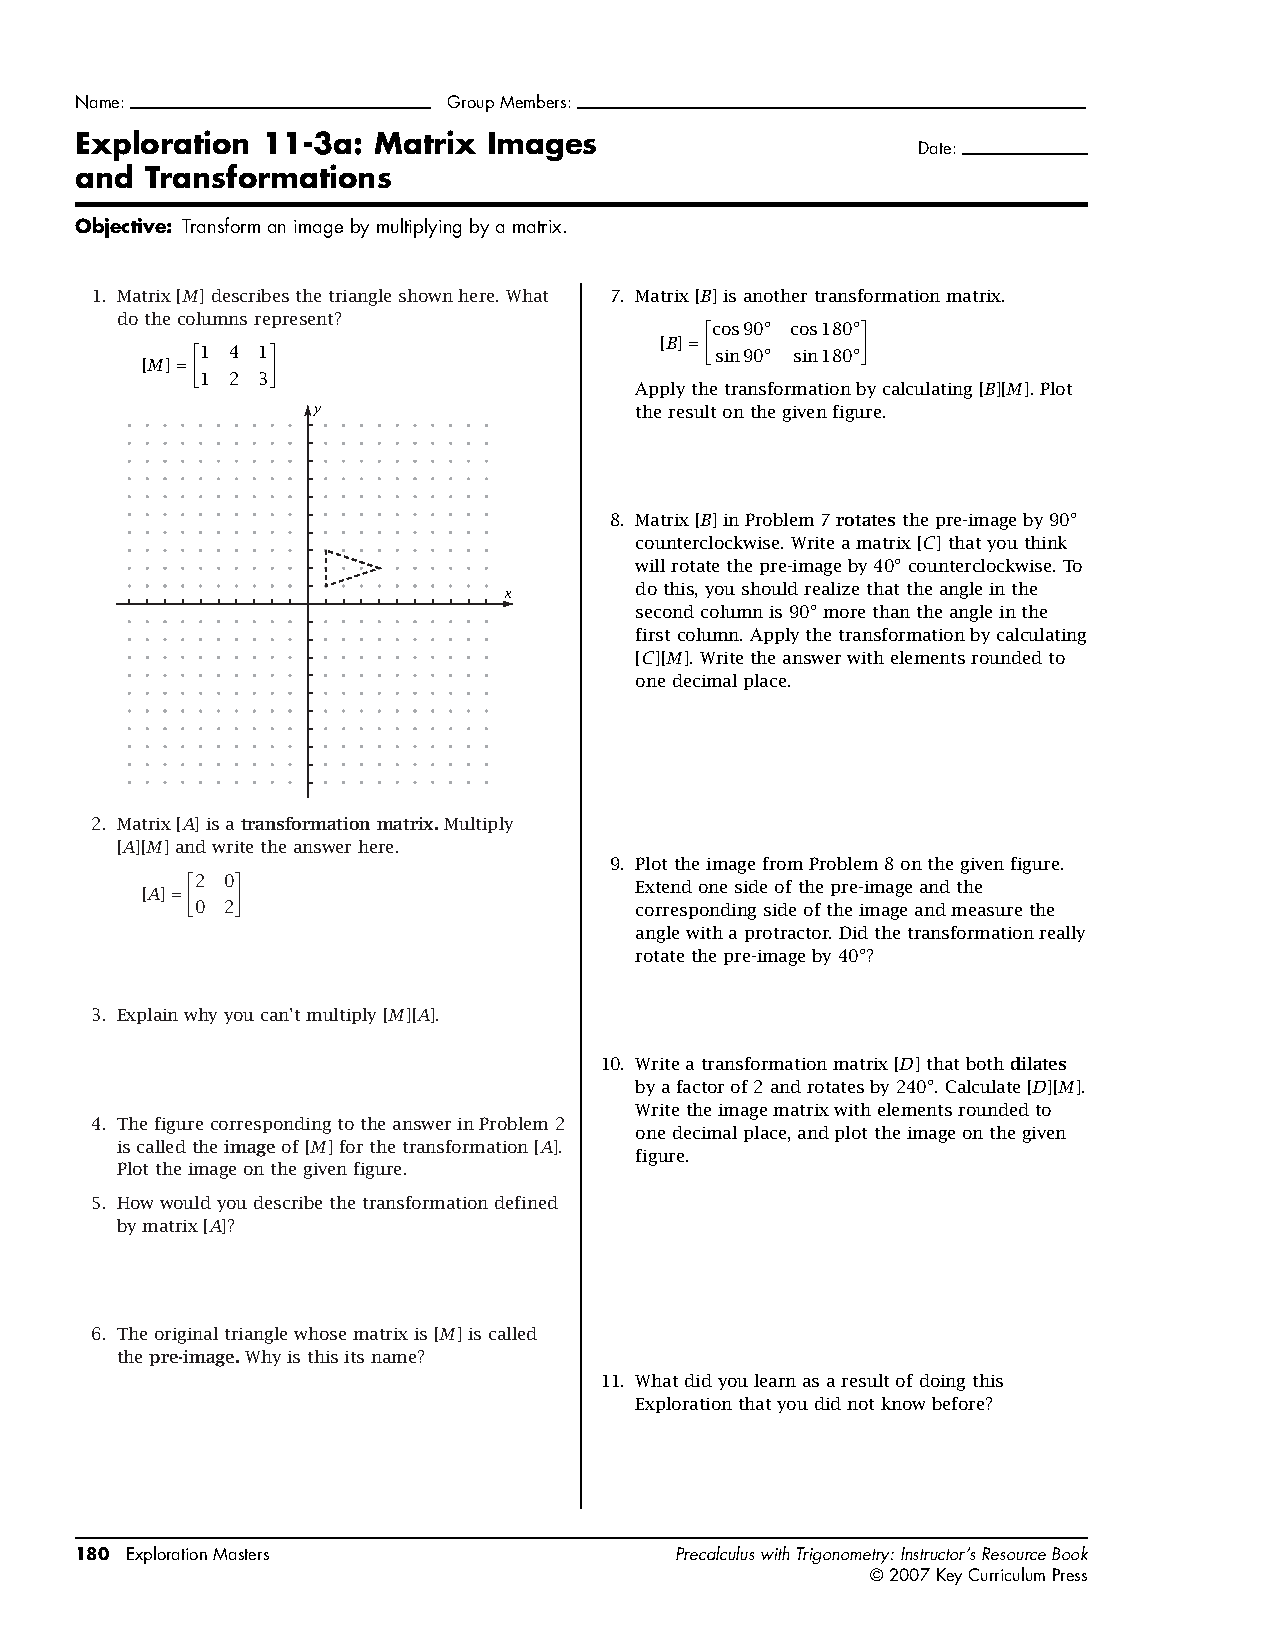
\includegraphics[width=\paperwidth]{chBB/BB01p.pdf}}
\subsection{Shifts}
\subsection{Reflections}
\subsection{Rotations}
\subsection{Derivatives}
\subsection{Exercises}

%									BB - 2
\newpage
\section{Walks}
\noindent\makebox[\textwidth]{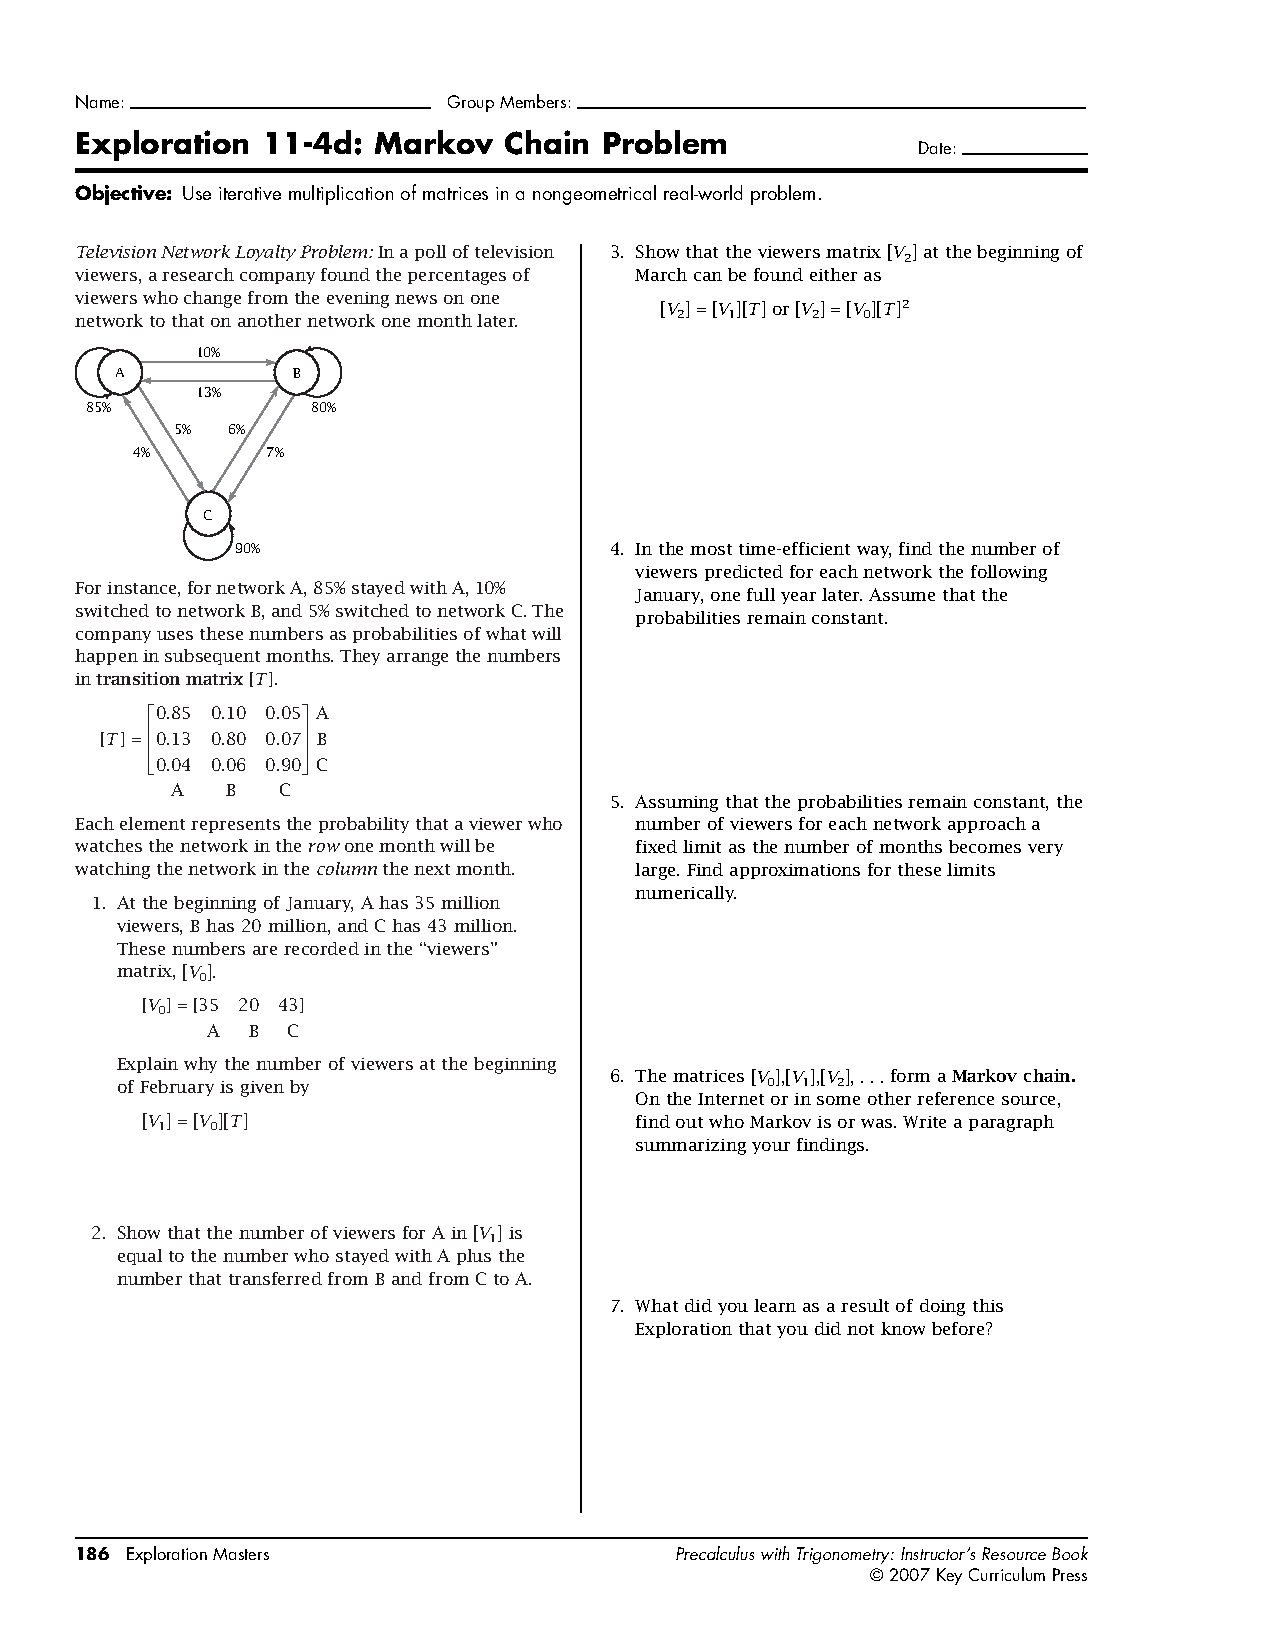
\includegraphics[width=\paperwidth]{chBB/BB02p.pdf}}
\subsection{Adjacency Maps}
\subsection{Unidirectional Lines}
\subsection{Exercises}

%									BB - 3
\newpage
\section{Vector-Spaces}
\subsection{Null Space}
\subsection{Dependent Systems}
\subsection{Exercises}

%									BB - 4
\newpage
\section{Determinants}
\subsection{Eigenvalues}
\subsection{Eigenvectors}
\subsection{Exercises}

%									BB - 5
\newpage
\section{Fractals}
\noindent\makebox[\textwidth]{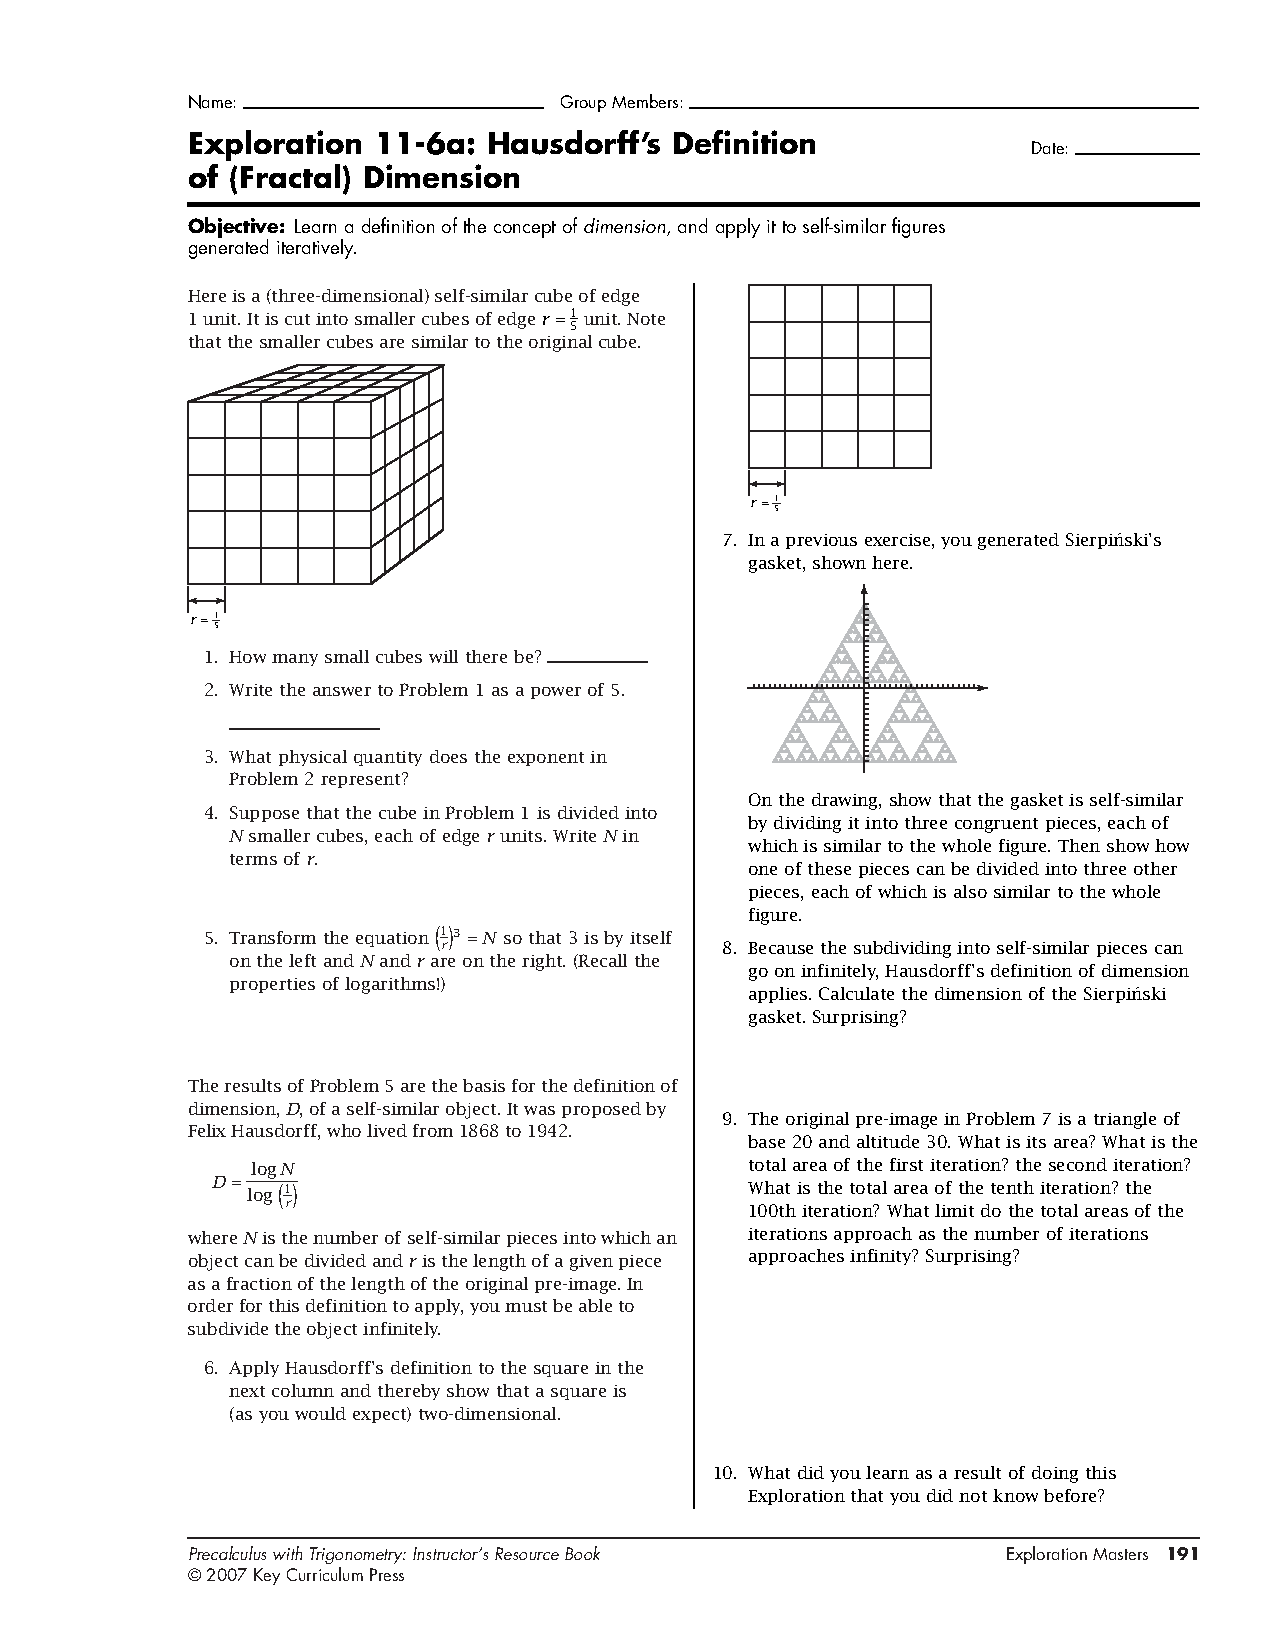
\includegraphics[width=\paperwidth]{chBB/BB05p.pdf}}
\newpage
\subsection{Text}
Nature is fractals, not smooth (locally linear) 
\newpage
\subsection{Exercises}
\noindent\makebox[\textwidth]{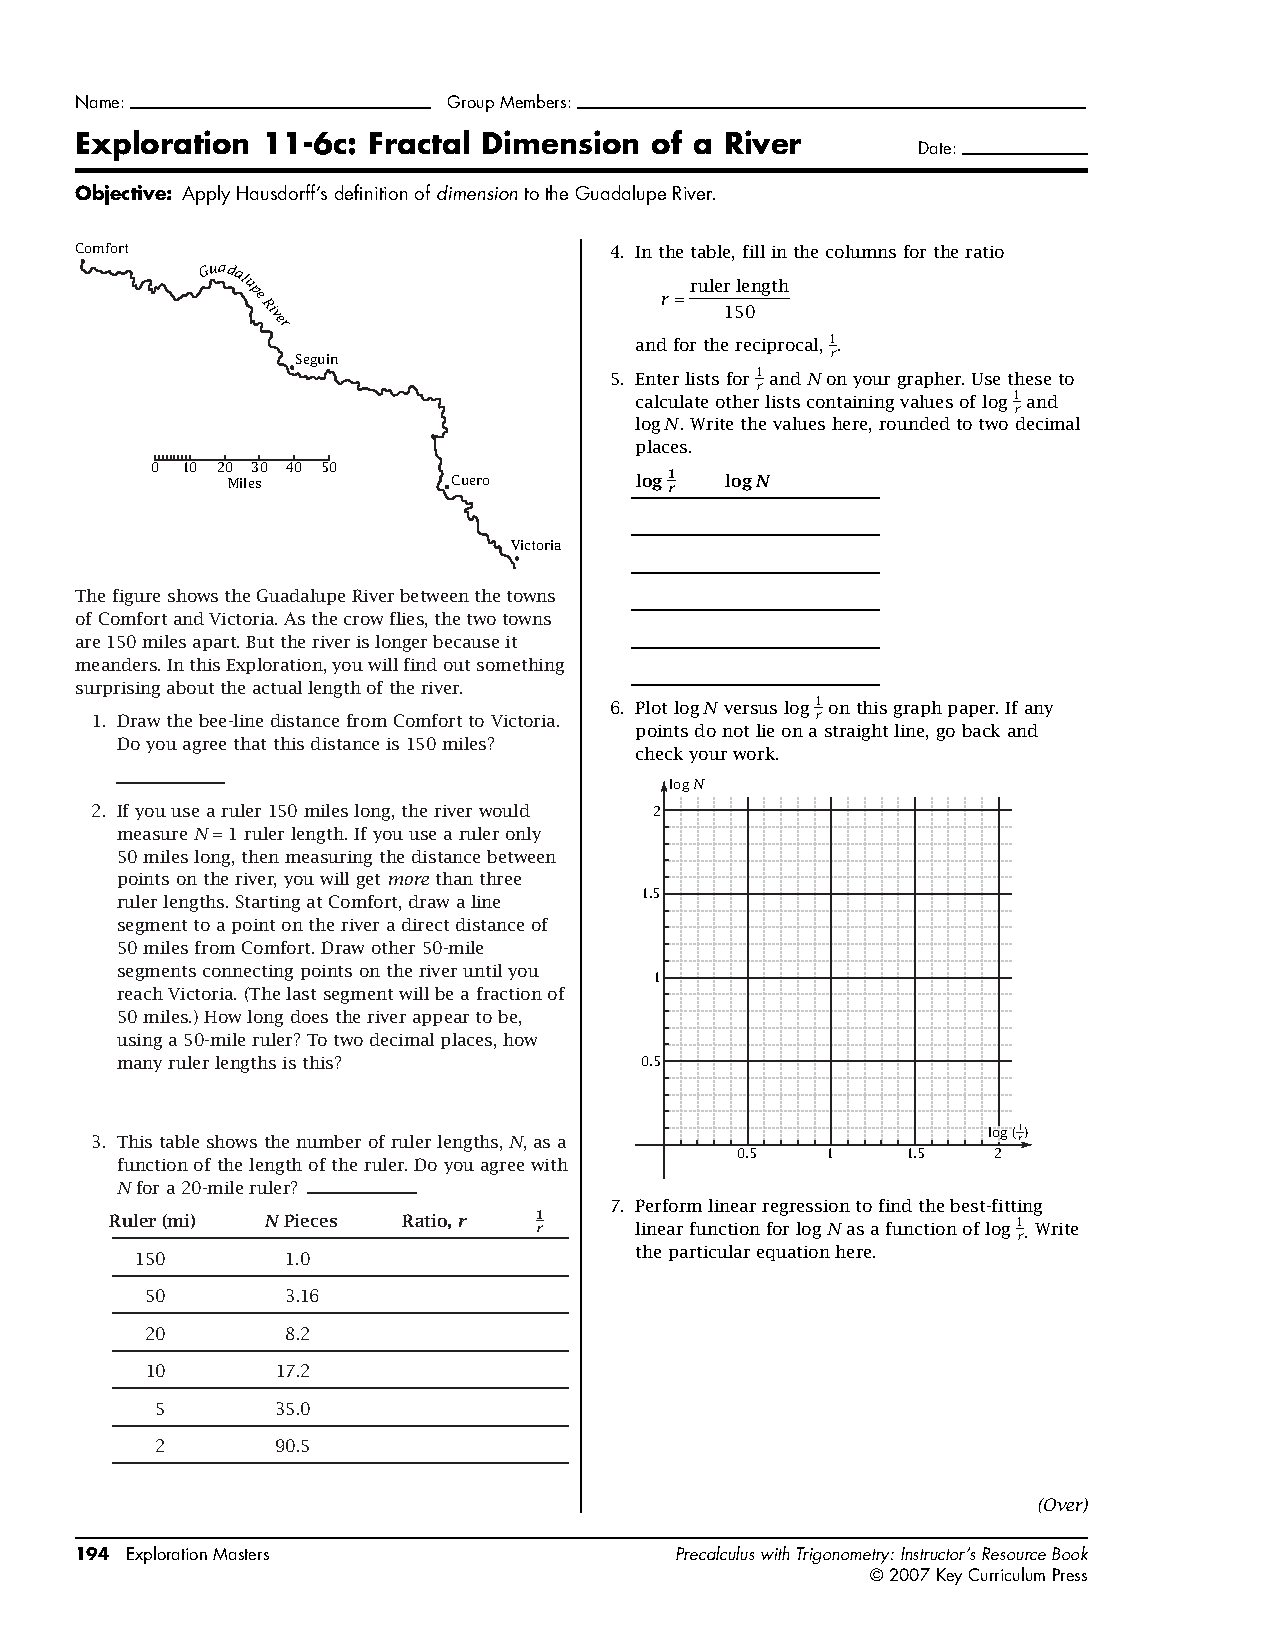
\includegraphics[width=\paperwidth]{chBB/BB05x.pdf}}


%									BB - 6
\newpage
\section{Review}
\subsection{Chapter Review}
\subsection{Chapter Test}